% Этот шаблон документа разработан в 2014 году
% Данилом Фёдоровых (danil@fedorovykh.ru) 
% для использования в курсе 
% <<Документы и презентации в \LaTeX>>, записанном НИУ ВШЭ
% для Coursera.org: http://coursera.org/course/latex .
% Исходная версия шаблона --- 
% https://www.writelatex.com/coursera/latex/3.2

\documentclass[a4paper,12pt]{article}

%%% Работа с русским языком
\usepackage{cmap}					% поиск в PDF
\usepackage{mathtext} 				% русские буквы в формулах
\usepackage[T2A]{fontenc}			% кодировка
\usepackage[utf8]{inputenc}			% кодировка исходного текста
\usepackage[english,russian]{babel}	% локализация и переносы

%%% Дополнительная работа с математикой
\usepackage{amsmath,amsfonts,amssymb,amsthm,mathtools} % AMS
\usepackage{icomma} % "Умная" запятая: $0,2$ --- число, $0, 2$ --- перечисление

%% Номера формул
%\mathtoolsset{showonlyrefs=true} % Показывать номера только у тех формул, на которые есть \eqref{} в тексте.
%\usepackage{leqno} % Нумерация формул слева

%% Свои команды
\DeclareMathOperator{\sgn}{\mathop{sgn}}

%% Перенос знаков в формулах (по Львовскому)
\newcommand*{\hm}[1]{#1\nobreak\discretionary{}
{\hbox{$\mathsurround=0pt #1$}}{}}

%%% Работа с картинками
\usepackage{graphicx}  % Для вставки рисунков
\graphicspath{{Materials/}{images2/}}  % папки с картинками
\setlength\fboxsep{3pt} % Отступ рамки \fbox{} от рисунка
\setlength\fboxrule{1pt} % Толщина линий рамки \fbox{}
\usepackage{wrapfig} % Обтекание рисунков текстом

%%% Работа с таблицами
\usepackage{array,tabularx,tabulary,booktabs} % Дополнительная работа с таблицами
\usepackage{longtable}  % Длинные таблицы
\usepackage{multirow} % Слияние строк в таблице

%%% Теоремы
\theoremstyle{plain} % Это стиль по умолчанию, его можно не переопределять.
\newtheorem{theorem}{Теорема}[section]
\newtheorem{proposition}[theorem]{Утверждение}
 
\theoremstyle{definition} % "Определение"
\newtheorem{corollary}{Следствие}[theorem]
\newtheorem{problem}{Задача}[section]
 
\theoremstyle{remark} % "Примечание"
\newtheorem*{nonum}{Решение}

%%% Программирование
\usepackage{etoolbox} % логические операторы

%%% Страница
%\usepackage{extsizes} % Возможность сделать 14-й шрифт
\usepackage{geometry} % Простой способ задавать поля
	\geometry{top=25mm}
	\geometry{bottom=35mm}
	\geometry{left=30mm}
	\geometry{right=20mm}
 %
\usepackage{fancyhdr} % Колонтитулы
 	\pagestyle{fancy}
 	\renewcommand{\headrulewidth}{0mm}  % Толщина линейки, отчеркивающей верхний колонтитул
 	\lfoot{}
 	\rfoot{}
 	\rhead{Верхний правый}
 	\chead{}
 	\lhead{ }
 	% \cfoot{Нижний в центре} % По умолчанию здесь номер страницы

\usepackage{setspace} % Интерлиньяж
%\onehalfspacing % Интерлиньяж 1.5
%\doublespacing % Интерлиньяж 2
%\singlespacing % Интерлиньяж 1

\usepackage{lastpage} % Узнать, сколько всего страниц в документе.

\usepackage{soulutf8} % Модификаторы начертания

\usepackage{hyperref}
\usepackage[usenames,dvipsnames,svgnames,table,rgb]{xcolor}
\hypersetup{				% Гиперссылки
    unicode=true,           % русские буквы в раздела PDF
    pdftitle={Заголовок},   % Заголовок
    pdfauthor={Автор},      % Автор
    pdfsubject={Тема},      % Тема
    pdfcreator={Создатель}, % Создатель
    pdfproducer={Производитель}, % Производитель
    pdfkeywords={keyword1} {key2} {key3}, % Ключевые слова
    colorlinks=true,       	% false: ссылки в рамках; true: цветные ссылки
    linkcolor=red,          % внутренние ссылки
    citecolor=green,        % на библиографию
    filecolor=magenta,      % на файлы
    urlcolor=cyan           % на URL
}

%\renewcommand{\familydefault}{\sfdefault} % Начертание шрифта

\usepackage{multicol} % Несколько колонок

% Мои "дополнительные" пакеты
\usepackage{textcase} 
\usepackage{pdfpages}
\usepackage{amsmath}


\author{Подкидышев Алексей}
\title{Студент МФТИ ФИВТ - 1ый курс}
\date{\today}

\begin{document} % конец преамбулы, начало документа

\thispagestyle{empty}
\begin{center}
	\textit{\MakeTextUppercase{федеральное государственное автономное учреждение}}
		
	\vspace{0.5ex}
	
	\textbf{ \\ \MakeTextUppercase{<<Московский Физико-технический институт>>}}
\end{center}
\vspace{13ex}
\begin{flushright}
	\noindent
	{Подкидышев Алексей Сергеевич}
	\\
	\textit{Студент факультета инноваций\\ и высоких технологий\\(группа 790)}
\end{flushright}
\begin{center}
	\vspace{23ex}
	{\LARGE\textbf{Лабораторная работа №2.5.1}}
	\vspace{1ex}
		
	\textbf{\large{<<Измерение коэффициента поверхностного натяжения>>}}
	
	\vfill
	Долгопрудный 
	
	{\today}
\end{center}

\newpage
\section{Установка} \label{sec:Inistal}
\subsection{Оборудование:}


\begin{wrapfigure}{l}{0.6\linewidth}\label{Pic1}
	\includegraphics[width=\linewidth]{Scheme.jpg}
	\caption{Схема установки}
\end{wrapfigure}Исследуемая жидкость (дистиллированная вода) наливается в сосуд (колбу) В (рис.1). Тестовая жидкость  (этиловый спирт) наливается  в сосуд Е.  При измерениях  колбы герметично закрываются  пробками.   Через одну из двух пробок  проходит полая металлическая игла С. Этой пробкой закрывается сосуд, в котором  проводятся измерения. Верхний конец иглы открыт в атмосферу, а нижний погружен в жидкость. Другой сосуд герметично закрывается второй пробкой. При создании достаточного  разряжения воздуха в колбе с иглой пузырьки воздуха начинают пробулькивать через жидкость. Поверхностное натяжение можно определить по величине разряжения $\vartriangle P$, необходимого для прохождения пузырьков (при известном радиусе иглы).
Разряжение в системе создается с помощью аспиратора А. Кран К2 разделяет две полости аспиратора. Верхняя полость при закрытом кране К2  заполняется водой. Затем кран К2 открывают и заполняют водой  нижнюю полость  аспиратора.  Разряжение воздуха создается в нижней полости  при открывании крана К1, когда  вода вытекает из неё по каплям. В колбах В и С, соединённых трубками с нижней полостью аспиратора,  создается такое же пониженное давление. Разность давлений в полостях с разряженным воздухом и атмосферой измеряется спиртовым микроманометром (устройство микроманометра описано в Приложении). 
Для стабилизации температуры исследуемой жидкости через рубашку D колбы В непрерывно прогоняется вода из термостата.

\subsection{Цель работы:}

\begin{itemize}
\item Измерение температурной зависимости  коэффициента поверхностного натяжения дистиллированной воды с использованием известного коэффициента поверхностного натяжения спирта; 
\item Определение полной поверхностной энергии  и теплоты, необходимой для изотермического образования единицы  поверхности жидкости  при различной температуре

\end{itemize}

\rhead{\large ~\nameref{sec:Inistal}}
	
\newpage
\section{Ход работы} \label{sec:MainWorks}

\rhead{\large ~\nameref{sec:MainWorks}}
\subsection{Измерение диаметра иглы:}
\begin{enumerate}
\item С помощью микроскопа:
\large{1,1 mm $\pm$ 0,1 mm}
\item С помощью помощью формулы Лапласа, предполагая $\sigma_\text{спирта} известным:$

\begin{tabular}{lllllll}
\cline{1-3}
\multicolumn{1}{|l|}{$P_0$, mm} & \multicolumn{1}{l|}{$P_0$, Па}  & \multicolumn{1}{l|}{$r_\text{иглы}$, mm}  &  &  &  &  \\ \cline{1-3}
\multicolumn{1}{|l|}{41,3}     & \multicolumn{1}{l|}{81,002929} & \multicolumn{1}{l|}{0,550597374} &  &  &  &  \\ \cline{1-3}
\end{tabular}
\end{enumerate}
Значения близки друг к другу. Возьмём среднее значение для \begin{Large}
$r_\text{иглы}$ = 0.55
\end{Large} 
mm. В дальнейшем будем считать, что радиус пузырьков воздуха будет равен полученному радиусу иглы.

\subsection{Измерения $h_1, h_2$:}
\begin{flushleft}
\textit{Перенесём предварительно промытую и 
просушенную от спирта иглу
в колбу с дистиллированной водой.} \\[1ex]
\end{flushleft}
\begin{itemize}
\item Измерим расстояние между верхним концом иглы и любой неподвижной часть прибора $h_1$(игла лишь касается поверхности)
\item Утопим иглу до предела и измерим $h_2$.
\[h_1 = 2.2 cm \ \ h_2 = 0.67 cm \Rightarrow \ \ \Delta H =1,53 cm\]
\end{itemize}

Измерим $\Delta H$ используя : \\[1ex]
\text{} \hspace{13ex} $\Delta p = \rho * g * h$
\begin{flushright}
\begin{tabular}{lllllll}
\cline{1-3}
\multicolumn{1}{|l|}{P1, Па} & \multicolumn{1}{l|}{P2, Па}    & \multicolumn{1}{l|}{$\Delta$H, cm}      &  &  &  &  \\ \cline{1-3}
\multicolumn{1}{|l|}{236,34} & \multicolumn{1}{l|}{398,14999} & \multicolumn{1}{l|}{1,651119643} &  &  &  &  \\ \cline{1-3}

\end{tabular}\\[3ex]

\textbf{Итого:}\\
Среднее значние \large{$\Delta$H = 1,59 cm}
\end{flushright}


\subsection{Измерение $\sigma(T)$ дистилированной воды:}
\[ \Delta P = \dfrac{2\sigma}{r} \hspace{1ex} \text{,где } \hspace{1ex} \Delta P = P - \rho*g*h_2\]
Воспользуемся этой формулой, так как $h_2$ - не зависит от температуры

\rhead{\large ~\nameref{sec:MainWorks}}
\includepdf{Graphics_Table.pdf}

\subsection{Измерение q}

\begin{tabular}{lllllllll}
\hline
\multicolumn{1}{|l|}{T} & \multicolumn{1}{l|}{295,5}   & \multicolumn{1}{l|}{303}     & \multicolumn{1}{l|}{308}     & \multicolumn{1}{l|}{313}     & \multicolumn{1}{l|}{318}     & \multicolumn{1}{l|}{323}     & \multicolumn{1}{l|}{328}     & \multicolumn{1}{l|}{333}     \\ \hline
\multicolumn{1}{|l|}{q} & \multicolumn{1}{l|}{52,4217} & \multicolumn{1}{l|}{53,7522} & \multicolumn{1}{l|}{54,6392} & \multicolumn{1}{l|}{55,5262} & \multicolumn{1}{l|}{56,4132} & \multicolumn{1}{l|}{57,3002} & \multicolumn{1}{l|}{58,1872} & \multicolumn{1}{l|}{59,0742} \\ \hline

\end{tabular}

\begin{figure}[h]
\center{\includegraphics[width=1\linewidth]{Yet.eps}}
\end{figure}

\subsection{Измерение F:}
\begin{tabular}{|l|l|l|l|l|l|l|l|l|}
\hline
T     & 295,5   & 303       & 308         & 313      & 318      & 323      & 328      & 333      \\ \hline
sigma & 66,6257 & 66,355977 & 65,16937254 & 64,19851 & 63,38947 & 62,31073 & 61,12413 & 60,53083 \\ \hline
U/F   & 119,047 & 120,10818 & 119,8085725 & 119,7247 & 119,8027 & 119,6109 & 119,3113 & 119,605  \\ \hline
\end{tabular}\\

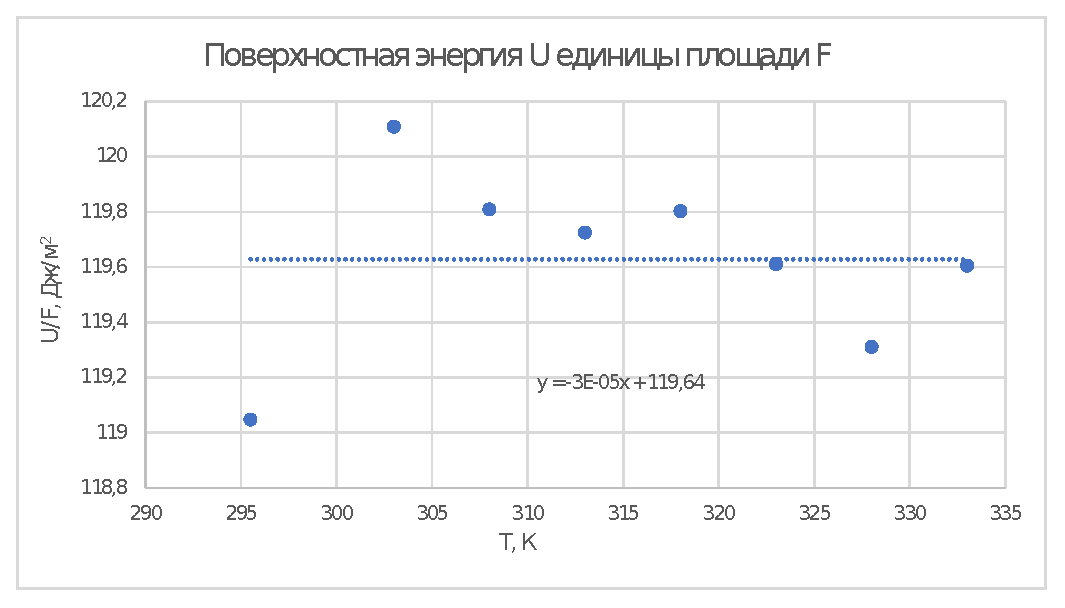
\includegraphics[width=1\linewidth]{FinalGraph.eps}
\subsubsection{Оценка полученных значений:}

\[\sigma_a =  \dfrac{1}{\sqrt{n}}\sqrt{\dfrac{\tilde{(y^2)} - (\tilde{y})^2 }{\tilde{x^2} - (\tilde{x})^2}- b^2} \]



Значение $\sigma_\text{a,b}$ для каждый коэфицентов составит:
\[\sigma_\text{a,b} \approx 17 \% \]

\section{Вывод}\label{sec:Vivod}


Используя данное оборудование, мы можем измерить коэффициент поверхностного натяжения жидкости и определить поверхностную энергию и теплоту образования единицы поверхности жидкости.
Полученные нами значения для коэфф. Поверхностного натяжения воды сходятся с табличными по порядку величины(относительная пошрешность 17$\%$):\\

\begin{tabular}{|l|l|l|}
\hline
$T^{\circ}$ &$\sigma_\text{воды}$ & Табличное значение \\ \hline
30      & 66,36         & 71,18     \\ \hline
40      & 64,2          & 69,56     \\ \hline
50      & 62,31         & 67,91     \\ \hline
\end{tabular}\\

Погрешность эксперимента объясняется неточностью приборов и самого процесса измерения: фиксация максимального давления «на глаз», отличие радиуса пузыря от радиуса иглы, температурное расширение металла иглы и неточность определения столба жидкости над иглой или момента касания поверхности.

\rhead{\large ~\nameref{sec:Vivod}}

\end{document} % конец документа

